% !TEX program = lualatex
        
% IMPORTANT! In order for the document to compile, one needs to use XeLaTeX or LuaLaTeX as compiler. This can be done in  Overleaf by Menu -> Settings -> Compiler -> Choose XeLaTeX/LuaLaTeX
\documentclass[t,24pt,aspectratio=169]{beamer}

\usepackage{UAM}
\usepackage{multicol} % Package for multiple coloumns
\usepackage[style=authoryear]{biblatex}
\usepackage{listings}
\usepackage{xcolor}

\definecolor{codegreen}{rgb}{0,0.6,0}
\definecolor{codegray}{rgb}{0.5,0.5,0.5}
\definecolor{codepurple}{rgb}{0.58,0,0.82}
\definecolor{backcolour}{rgb}{0.95,0.95,0.92}

\lstset{
	backgroundcolor=\color{backcolour},
	commentstyle=\color{codegreen},
	keywordstyle=\color{magenta},
	numberstyle=\tiny\color{codegray},
	stringstyle=\color{codepurple},
	basicstyle=\ttfamily\footnotesize,
	breaklines=true,
	frame=single,
	showstringspaces=false
}

%\usepackage{minted}
% lualatex -shell-escape -synctex=1 -interaction=nonstopmode archivo.tex

% \toplinje{Text at top} % The text at top. Remove the command if no text is desired


\addbibresource{references.bib}
\begin{document}

% The first slide. One can for instance change the main title, the subtitle, speaker, KU-unit, date and backgroundimage
{
\setbeamertemplate{background}{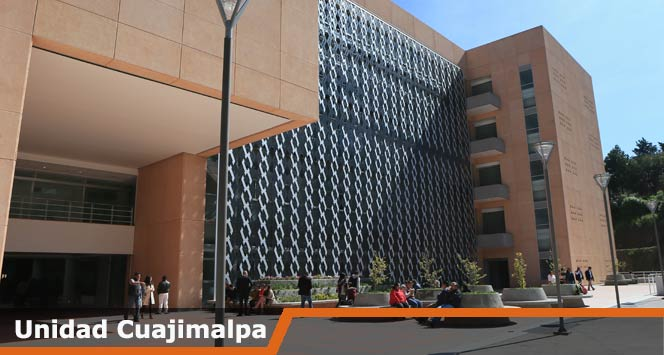
\includegraphics[width=\paperwidth,height=\paperheight]{uam/cua_05.jpg}}
\begin{frame}
    \begin{textblock*}{\textwidth}(0.53\textwidth,0.1\textheight)
        \begin{beamercolorbox}[wd=8.5cm,ht=7.3cm,sep=0.5cm]{hvidbox}
            \fontsize{5}{10}\fontfamily{ptm}\selectfont \textls[200]{UNIVERSIDAD AUTÓNOMA METROPOLITANA}
            \noindent\textcolor{KUrod}{\rule{6.8cm}{0.4pt}}
        \end{beamercolorbox}
    \end{textblock*}
    \begin{textblock*}{\textwidth}(0.53\textwidth,0.1\textheight)
        \begin{beamercolorbox}[wd=8.5cm,sep=0.5cm]{hvidbox}
                \Huge \textcolor{KUrod}{Integración de sistemas}
                \vspace{0.5cm}
                \par
                \Large Integración Formal, Tipos de integración

                \vspace{0.5cm}
                \par
                \normalsize Juan Alvarado
        \end{beamercolorbox}
    \end{textblock*}
    \begin{textblock}{1}(14.5,11.38)
        % \includegraphics[width=1cm]{KU/KU-logo.png}
    \end{textblock}
\end{frame}
}


        %%%%%%%%%%%%%%%%%%%%%%%%%%%%%%%%%%%%%%%
	\begin{frame}[fragile, hvid]
		\frametitle{Visión general de la integración}
			\vfill
			\centering
			\Huge{Visión general de la integración}
			\vfill
	\end{frame}
%%%%%%%%%%%%%%%%%%%%%%%%%%%%%%%%%%%%%%%


%%%%%%%%%%%%%%%%%%%%%%%%%%%%%%%%%%%%%%%
	\begin{frame}[fragile, hvid]
		\frametitle{Visión general de la integración}
			\vfill
\begin{multicols}{2} 

En una organización típica conviven múltiples aplicaciones: ERP, CRM, portal web, apps móviles, sistemas legados, etc., cada una con su propia base de datos y lógica de negocio.
\\~\\
\columnbreak
\centering

\includegraphics[width=6.6cm,height=5.9cm,keepaspectratio]{img/thumbs_up.jpg}
\end{multicols}
			\vfill
	\end{frame}
%%%%%%%%%%%%%%%%%%%%%%%%%%%%%%%%%%%%%%%


%%%%%%%%%%%%%%%%%%%%%%%%%%%%%%%%%%%%%%%
	\begin{frame}[fragile, hvid]
		\frametitle{Visión general de la integración}
			\vfill
La \textbf{integración} de sistemas busca que todos esos componentes se coordinen como si fueran un solo sistema coherente, sin que el usuario tenga que saber qué aplicación está "detrás" de cada operación.
\\~\\
			\vfill
	\end{frame}
%%%%%%%%%%%%%%%%%%%%%%%%%%%%%%%%%%%%%%%


%%%%%%%%%%%%%%%%%%%%%%%%%%%%%%%%%%%%%%%
	\begin{frame}[fragile, hvid]
		\frametitle{Visión general de la integración}
			\vfill
\begin{multicols}{2} 

Esto implica que los sistemas puedan intercambiar datos, invocar funciones remotas y compartir una interpretación común de la información clave del negocio.
\\~\\
\columnbreak
\centering

\includegraphics[width=6.6cm,height=5.9cm,keepaspectratio]{img/pexels-thisisengineering-3861951.jpg}
\end{multicols}
			\vfill
	\end{frame}
%%%%%%%%%%%%%%%%%%%%%%%%%%%%%%%%%%%%%%%


%%%%%%%%%%%%%%%%%%%%%%%%%%%%%%%%%%%%%%%
	\begin{frame}[fragile, hvid]
		\frametitle{Tipos de integración: datos, funcional y semántica}
			\vfill
			\centering
			\Huge{Tipos de integración: datos, funcional y semántica}
			\vfill
	\end{frame}
%%%%%%%%%%%%%%%%%%%%%%%%%%%%%%%%%%%%%%%


%%%%%%%%%%%%%%%%%%%%%%%%%%%%%%%%%%%%%%%
	\begin{frame}[fragile, hvid]
		\frametitle{Tipos de integración: datos, funcional y semántica}
			\vfill
Hay tres categorías básicas para clasificar los problemas de integración.
\\~\\
- \textbf{Integración de datos}: cuando el reto principal es mover o sincronizar datos entre fuentes distintas, como bases relacionales, archivos planos o APIs de terceros.
\\~\\
			\vfill
	\end{frame}
%%%%%%%%%%%%%%%%%%%%%%%%%%%%%%%%%%%%%%%


%%%%%%%%%%%%%%%%%%%%%%%%%%%%%%%%%%%%%%%
	\begin{frame}[fragile, hvid]
		\frametitle{Tipos de integración: datos, funcional y semántica}
			\vfill
\begin{multicols}{2} 

- \textbf{Integración funcional}: cuando el objetivo es coordinar funciones o servicios de sistemas diferentes para construir procesos de negocio completos, por ejemplo, un flujo de "pago en línea" que llama a un procesador bancario externo.
\\~\\
\columnbreak
\centering

\includegraphics[width=6.6cm,height=5.9cm,keepaspectratio]{img/pexels-pixabay-208494.jpg}
\end{multicols}
			\vfill
	\end{frame}
%%%%%%%%%%%%%%%%%%%%%%%%%%%%%%%%%%%%%%%


%%%%%%%%%%%%%%%%%%%%%%%%%%%%%%%%%%%%%%%
	\begin{frame}[fragile, hvid]
		\frametitle{Tipos de integración: datos, funcional y semántica}
			\vfill
\begin{multicols}{2} 

- \textbf{Integración semántica}: cuando hay que alinear el significado de los datos, resolviendo diferencias en vocabulario, estructura o modelos conceptuales entre aplicaciones.
\\~\\
\columnbreak
\centering

\includegraphics[width=6.6cm,height=5.9cm,keepaspectratio]{img/pexels-roman-odintsov-6898856.jpg}
\end{multicols}
			\vfill
	\end{frame}
%%%%%%%%%%%%%%%%%%%%%%%%%%%%%%%%%%%%%%%


%%%%%%%%%%%%%%%%%%%%%%%%%%%%%%%%%%%%%%%
	\begin{frame}[fragile, hvid]
		\frametitle{Integración de datos}
			\vfill
			\centering
			\Huge{Integración de datos}
			\vfill
	\end{frame}
%%%%%%%%%%%%%%%%%%%%%%%%%%%%%%%%%%%%%%%


%%%%%%%%%%%%%%%%%%%%%%%%%%%%%%%%%%%%%%%
	\begin{frame}[fragile, hvid]
		\frametitle{Integración de datos}
			\vfill
La integración de \textbf{datos} se centra en unificar información dispersa para que se pueda consultar o analizar como un todo.
\\~\\
			\vfill
	\end{frame}
%%%%%%%%%%%%%%%%%%%%%%%%%%%%%%%%%%%%%%%


%%%%%%%%%%%%%%%%%%%%%%%%%%%%%%%%%%%%%%%
	\begin{frame}[fragile, hvid]
		\frametitle{Integración de datos}
			\vfill
\begin{multicols}{2} 

Esto incluye tareas como consolidar catálogos de clientes que están duplicados en varios sistemas, o mantener sincronizados inventarios entre la tienda en línea y el sistema de almacén.
\\~\\
\columnbreak
\centering
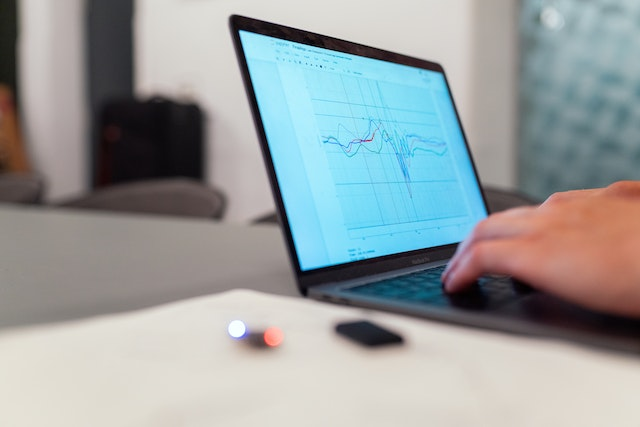
\includegraphics[width=6.6cm,height=5.9cm,keepaspectratio]{img/pexels-thisisengineering-3912976.jpg}
\end{multicols}
			\vfill
	\end{frame}
%%%%%%%%%%%%%%%%%%%%%%%%%%%%%%%%%%%%%%%


%%%%%%%%%%%%%%%%%%%%%%%%%%%%%%%%%%%%%%%
	\begin{frame}[fragile, hvid]
		\frametitle{Integración de datos}
			\vfill
Las soluciones típicas incluyen procesos ETL (Extract, Transform, Load), replicación de bases de datos y APIs de lectura/escritura que exponen vistas unificadas.
\\~\\
			\vfill
	\end{frame}
%%%%%%%%%%%%%%%%%%%%%%%%%%%%%%%%%%%%%%%


%%%%%%%%%%%%%%%%%%%%%%%%%%%%%%%%%%%%%%%
	\begin{frame}[fragile, hvid]
		\frametitle{Integración de datos}
			\vfill
\begin{multicols}{2} 

Aquí nos interesa distinguir cuándo el problema principal es “datos incoherentes” frente a otros tipos de problemas de integración.
\\~\\
\columnbreak
\centering

\includegraphics[width=6.6cm,height=5.9cm,keepaspectratio]{img/pexels-arthur-brognoli-2440530.jpg}
\end{multicols}
			\vfill
	\end{frame}
%%%%%%%%%%%%%%%%%%%%%%%%%%%%%%%%%%%%%%%


%%%%%%%%%%%%%%%%%%%%%%%%%%%%%%%%%%%%%%%
	\begin{frame}[fragile, hvid]
		\frametitle{Actividad: Mapa rápido de integraciones de datos}
			\vfill
En equipos, elijan un contexto cercano (la universidad, un e‑commerce simple, un hospital pequeño).
\\~\\
			\vfill
	\end{frame}
%%%%%%%%%%%%%%%%%%%%%%%%%%%%%%%%%%%%%%%


%%%%%%%%%%%%%%%%%%%%%%%%%%%%%%%%%%%%%%%
	\begin{frame}[fragile, hvid]
		\frametitle{Actividad: Mapa rápido de integraciones de datos}
			\vfill
\begin{multicols}{2} 

Enumeren al menos cinco sistemas o aplicaciones que podrían existir en ese contexto y dibujen flechas cuando haya un intercambio de datos claro (por ejemplo, calificaciones de un LMS hacia el sistema institucional).
\\~\\
\columnbreak
\centering

\includegraphics[width=6.6cm,height=5.9cm,keepaspectratio]{img/pexels-olya-kobruseva-5428836.jpg}
\end{multicols}
			\vfill
	\end{frame}
%%%%%%%%%%%%%%%%%%%%%%%%%%%%%%%%%%%%%%%


%%%%%%%%%%%%%%%%%%%%%%%%%%%%%%%%%%%%%%%
	\begin{frame}[fragile, hvid]
		\frametitle{Actividad: Mapa rápido de integraciones de datos}
			\vfill
\begin{multicols}{2} 

Marquen con un color las flechas donde el \textbf{principal reto sería que los datos sean consistentes} (mismo alumno, mismos IDs, mismas fechas).
\\~\\
\columnbreak
\centering
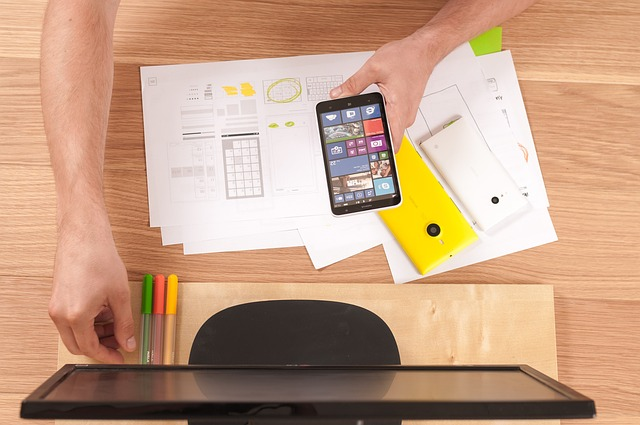
\includegraphics[width=6.6cm,height=5.9cm,keepaspectratio]{img/phone-g29857e29e_640.jpg}
\end{multicols}
			\vfill
	\end{frame}
%%%%%%%%%%%%%%%%%%%%%%%%%%%%%%%%%%%%%%%


%%%%%%%%%%%%%%%%%%%%%%%%%%%%%%%%%%%%%%%
	\begin{frame}[fragile, hvid]
		\frametitle{Integración funcional}
			\vfill
			\centering
			\Huge{Integración funcional}
			\vfill
	\end{frame}
%%%%%%%%%%%%%%%%%%%%%%%%%%%%%%%%%%%%%%%


%%%%%%%%%%%%%%%%%%%%%%%%%%%%%%%%%%%%%%%
	\begin{frame}[fragile, hvid]
		\frametitle{Integración funcional}
			\vfill
\begin{multicols}{2} 

La integración \textbf{funcional} se trata de coordinar capacidades de distintos sistemas para lograr un flujo de negocio completo.
\\~\\
\columnbreak
\centering

\includegraphics[width=6.6cm,height=5.9cm,keepaspectratio]{img/important-g74dfdc749_640.png}
\end{multicols}
			\vfill
	\end{frame}
%%%%%%%%%%%%%%%%%%%%%%%%%%%%%%%%%%%%%%%


%%%%%%%%%%%%%%%%%%%%%%%%%%%%%%%%%%%%%%%
	\begin{frame}[fragile, hvid]
		\frametitle{Integración funcional}
			\vfill
Por ejemplo, un flujo de "compra en línea" puede orquestar funciones de catálogo, carrito, pagos, facturación y envío, cada una ofrecida por sistemas diferentes.
\\~\\
			\vfill
	\end{frame}
%%%%%%%%%%%%%%%%%%%%%%%%%%%%%%%%%%%%%%%


%%%%%%%%%%%%%%%%%%%%%%%%%%%%%%%%%%%%%%%
	\begin{frame}[fragile, hvid]
		\frametitle{Integración funcional}
			\vfill
En este escenario, el foco no está solo en copiar datos, sino en invocar operaciones remotas (servicios) con entradas y salidas bien definidas.
\\~\\
Estilos como SOA y microservicios son variaciones de cómo organizar esa integración funcional.
\\~\\
			\vfill
	\end{frame}
%%%%%%%%%%%%%%%%%%%%%%%%%%%%%%%%%%%%%%%


%%%%%%%%%%%%%%%%%%%%%%%%%%%%%%%%%%%%%%%
	\begin{frame}[fragile, hvid]
		\frametitle{Integración semántica}
			\vfill
			\centering
			\Huge{Integración semántica}
			\vfill
	\end{frame}
%%%%%%%%%%%%%%%%%%%%%%%%%%%%%%%%%%%%%%%


%%%%%%%%%%%%%%%%%%%%%%%%%%%%%%%%%%%%%%%
	\begin{frame}[fragile, hvid]
		\frametitle{Integración semántica}
			\vfill
\begin{multicols}{2} 

La integración \textbf{semántica} intenta resolver el problema de que “no hablamos el mismo idioma” aunque los sistemas intercambien datos.
\\~\\
\columnbreak
\centering
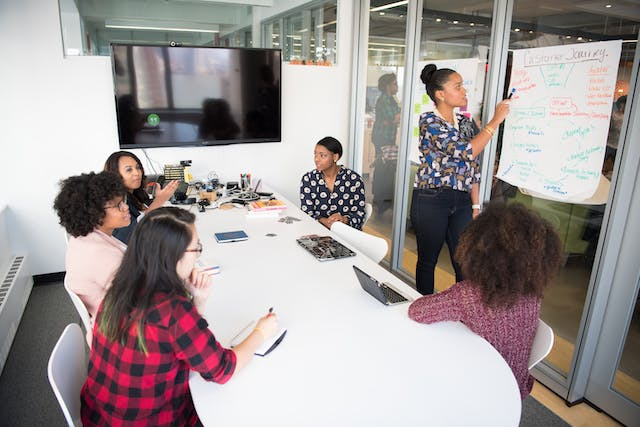
\includegraphics[width=6.6cm,height=5.9cm,keepaspectratio]{img/pexels-christina-morillo-1181622.jpg}
\end{multicols}
			\vfill
	\end{frame}
%%%%%%%%%%%%%%%%%%%%%%%%%%%%%%%%%%%%%%%


%%%%%%%%%%%%%%%%%%%%%%%%%%%%%%%%%%%%%%%
	\begin{frame}[fragile, hvid]
		\frametitle{Integración semántica}
			\vfill
\begin{multicols}{2} 

Dos aplicaciones pueden usar el campo “clave\_producto” con significados distintos, o representar direcciones, productos o diagnósticos médicos con modelos incompatibles.
\\~\\
\columnbreak
\centering

\includegraphics[width=6.6cm,height=5.9cm,keepaspectratio]{img/reminder-g3c09298ed_640.png}
\end{multicols}
			\vfill
	\end{frame}
%%%%%%%%%%%%%%%%%%%%%%%%%%%%%%%%%%%%%%%


%%%%%%%%%%%%%%%%%%%%%%%%%%%%%%%%%%%%%%%
	\begin{frame}[fragile, hvid]
		\frametitle{Integración semántica}
			\vfill
Las técnicas semánticas introducen modelos compartidos (ontologías, vocabularios controlados, esquemas bien definidos) para que el dato pueda interpretarse de la misma manera en contextos diferentes.
\\~\\
			\vfill
	\end{frame}
%%%%%%%%%%%%%%%%%%%%%%%%%%%%%%%%%%%%%%%


%%%%%%%%%%%%%%%%%%%%%%%%%%%%%%%%%%%%%%%
	\begin{frame}[fragile, hvid]
		\frametitle{Integración semántica}
			\vfill
\begin{multicols}{2} 

Es importante reconocer que sin una capa semántica, integrar solo por campos y tipos puede generar errores sutiles.
\\~\\
\columnbreak
\centering

\includegraphics[width=6.6cm,height=5.9cm,keepaspectratio]{img/pexels-marc-mueller-380769.jpg}
\end{multicols}
			\vfill
	\end{frame}
%%%%%%%%%%%%%%%%%%%%%%%%%%%%%%%%%%%%%%%


%%%%%%%%%%%%%%%%%%%%%%%%%%%%%%%%%%%%%%%
	\begin{frame}[fragile, hvid]
		\frametitle{Relación entre los tres tipos}
			\vfill
			\centering
			\Huge{Relación entre los tres tipos}
			\vfill
	\end{frame}
%%%%%%%%%%%%%%%%%%%%%%%%%%%%%%%%%%%%%%%


%%%%%%%%%%%%%%%%%%%%%%%%%%%%%%%%%%%%%%%
	\begin{frame}[fragile, hvid]
		\frametitle{Relación entre los tres tipos}
			\vfill
En proyectos reales, los tres tipos de integración aparecen mezclados.
\\~\\
			\vfill
	\end{frame}
%%%%%%%%%%%%%%%%%%%%%%%%%%%%%%%%%%%%%%%


%%%%%%%%%%%%%%%%%%%%%%%%%%%%%%%%%%%%%%%
	\begin{frame}[fragile, hvid]
		\frametitle{Relación entre los tres tipos}
			\vfill
\begin{multicols}{2} 

Un portal de autoservicio para clientes puede requerir: datos integrados (historial de compras), funciones integradas (proceso de pago y entrega) y semántica común (qué significa “cliente activo”, “pedido entregado” o “saldo vencido”).
\\~\\
\columnbreak
\centering

\includegraphics[width=6.6cm,height=5.9cm,keepaspectratio]{img/pexels-pixabay-356079.jpg}
\end{multicols}
			\vfill
	\end{frame}
%%%%%%%%%%%%%%%%%%%%%%%%%%%%%%%%%%%%%%%


%%%%%%%%%%%%%%%%%%%%%%%%%%%%%%%%%%%%%%%
	\begin{frame}[fragile, hvid]
		\frametitle{Relación entre los tres tipos}
			\vfill
\begin{multicols}{2} 

Identificar explícitamente qué tipo de integración predomina en cada parte del proyecto ayuda a elegir tecnologías y estrategias adecuadas, como priorizar mapeos de datos, orquestación de servicios o alineación de vocabularios.
\\~\\
\columnbreak
\centering

\includegraphics[width=6.6cm,height=5.9cm,keepaspectratio]{img/pexels-arthur-brognoli-2440530.jpg}
\end{multicols}
			\vfill
	\end{frame}
%%%%%%%%%%%%%%%%%%%%%%%%%%%%%%%%%%%%%%%


%%%%%%%%%%%%%%%%%%%%%%%%%%%%%%%%%%%%%%%
	\begin{frame}[fragile, hvid]
		\frametitle{Práctica}
			\vfill
			\centering
			\Huge{Práctica}
			\vfill
	\end{frame}
%%%%%%%%%%%%%%%%%%%%%%%%%%%%%%%%%%%%%%%


%%%%%%%%%%%%%%%%%%%%%%%%%%%%%%%%%%%%%%%
	\begin{frame}[fragile, hvid]
		\frametitle{Práctica}
			\vfill
\textbf{Detectando tipos de integración en un caso sencillo}
\\~\\
En esta práctica se analizará un escenario de una pequeña empresa y se etiquetarán las necesidades de integración como de datos, funcionales o semánticas.
\\~\\
			\vfill
	\end{frame}
%%%%%%%%%%%%%%%%%%%%%%%%%%%%%%%%%%%%%%%


%%%%%%%%%%%%%%%%%%%%%%%%%%%%%%%%%%%%%%%
	\begin{frame}[fragile, hvid]
		\frametitle{Práctica}
			\vfill
El trabajo se puede realizar con herramientas colaborativas digitales.
\\~\\
			\vfill
	\end{frame}
%%%%%%%%%%%%%%%%%%%%%%%%%%%%%%%%%%%%%%%


{
	\setbeamertemplate{background}{
\includegraphics[width=\paperwidth,height=\paperheight]{uam/cua_01.jpg}}
	\begin{frame}[billede]
		\begin{textblock*}{\textwidth}(0\textwidth,0.77\textheight)
			\begin{beamercolorbox}[wd=7.8cm,sep=0.3cm]{rodbox}
				{\huge ¡Gracias!}
			\end{beamercolorbox}
		\end{textblock*}
	\end{frame}
}

%%%%% THIS IS THE BLOCK OF REFERENCES 

% \begin{frame}[hvid, allowframebreaks]
	% \frametitle{Referencias}
	% \printbibliography
	
	% \end{frame}


%%%%%% END OF THE BLOCK OF REFERENCES

\end{document}
